%
% LaTeX report template 
%
\documentclass[a4paper,10pt]{article}
\usepackage{graphicx}
\usepackage[english]{babel}
\usepackage[latin1]{inputenc}
\usepackage{amsfonts}
%
\begin{document}
%
   \title{Probabilistic Matrix Analysis}

   \author{ Hekmat Taherinejad, Rahim Tariverdi, Hamidreza Behjoo, Kodirjon Akhmedov}
          
   \date{\today}

   \maketitle
   
   \tableofcontents
 
  \newpage
    
% This is a comment: in LaTeX everything that in a line comes
% after a "%" symbol is treated as comment
\section{Appetizer}
% When adding * to \section, \subsection, etc... LaTeX will not assign
% a number to the section
Singular Value Decomposition (SVD) is a useful framework for dimensionality reduction tasks. Consider Principal Component Analysis (PCA), which, given a centered matrix of $m$ observations and $p$ covariates $X \in R^{m \times p}$, computes $W \in R^{p \times l}$ and $\Lambda \in R^{l \times l}$ such that $X^T X \approx W \Lambda W^T$. This maps the original observations from a $p$-dimensional space into an $l$-dimensional space, for $l \leq p$, thus performing dimensionality reduction. One algorithm for computing a reduced PCA is via a low-rank matrix approximation. Take $X \approx U_r \Sigma_r V_r ^T$, and then take $X^T X \approx (U_r \Sigma_r V_r^T)^{T} (U_r \Sigma_r V_r^T) = V_r \Sigma_r ^2 V_r^T$ by the orthogonality of $U_r$. Thus computing the SVD of $A$ immediately yields the PCA of $A$.\\

These techniques have a huge number of applications in machine learning, data mining, bioinformatics, and even political science -- from predicting hashtags from the content of a status by factorizing their co-occurrence matrix, to understanding political voting patterns by factorizing the matrix of legislators and bills.

Unfortunately, computing the SVD can be extremely time-consuming for the large-scale problems. Thus, we turn to randomized methods which offer significant speedups over classical methods.


\section{Introduction}
Indeed, matrix decompositions are often the workhorse algorithms for scientific computing applications in the areas of applied mathematics, statistical computing, and machine learning. Despite our ever-increasing computational power, the emergence of large-scale datasets has severely challenged our ability to analyze data using traditional matrix algorithms. Moreover, the growth of data collection is far outstripping computational performance gains. The computationally expensive singular value decomposition (SVD) is the most ubiquitous method for dimensionality reduction, data processing and compression. The concept of randomness has recently been demonstrated as an effective strategy to easing the computational demands of low-rank approximations from matrix decompositions such as the SVD, thus allowing for a scalable architecture for modern big data applications.

The basic idea of probabilistic matrix algorithms is to employ a degree of randomness in order to derive a smaller matrix from a high-dimensional matrix, which captures the essential information. Thus, none of the randomnes should obscure the dominant spectral information of the data as long as the input matrix features some low-rank structure. Then, a deterministic matrix factorization algorithm is applied to the smaller matrix to compute a near-optimal low-rank approximation. The principal concept is sketched in Figure 1.

\begin{figure}
	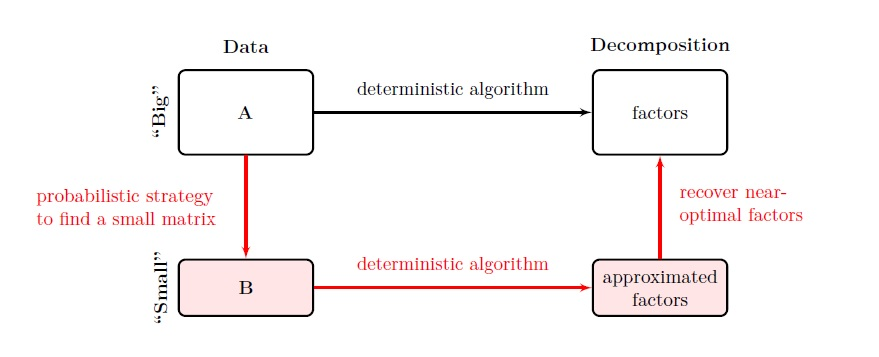
\includegraphics[scale=0.5]{fig1.jpg}
	\caption{First, randomness is used as a computational strategy to derive a smaller matrix
		$B$ from $A$. Then, the low-dimensional matrix is used to compute an approximate matrix
		decomposition. Finally, the near-optimal (high-dimensional) factors may be reconstructed.}
	\label{fig1}
\end{figure}


\section{Probabilistic framework for low-rank approximations}
In the following, we advocate the probabilistic framework, formulated by Halko et al. (2011), to compute a near-optimal low-rank approximation. Conceptually, this framework splits the computational task into two logical stages:

\begin{itemize}
	\item Stage A: Construct a low dimensional subspace that approximates the column space of $A$. This means, the aim is to find a matrix $Q \in R^{m\times k}$ with orthonormal columns such that  $A\approx QQTA$ is satisfied.
	
	\item Stage B: Form a smaller matrix $B=Q^T A \in R^{k \times n}$, i.e., restrict the high-dimensional
	input matrix to the low-dimensional space spanned by the near-optimal basis $Q$. The
	smaller matrix $B$ can then be used to compute a desired low-rank approximation.
	
\end{itemize}

The first computational stage is where randomness comes into the play, while the second stage is  purely deterministic. In the following, the two stages are described in detail.

\subsection{The generic randomized algorithm}

\textit{Stage A: Computing the near-optimal basis} 

First, we aim to find a near-optimal basis Q for the matrix A such that $A \approx QQ^T A$ is satisfied. The desired target rank k is assumed to be $k \ll \min{(m, n)}$. Specifically, $P := QQ^T$ is a linear orthogonal projector. A projection operator corresponds to a linear subspace, and transforms any vector to its orthogonal projection on the subspace. This is illustrated in Figure 2, where a vector x is confined to the column space col(A).

\begin{figure}
	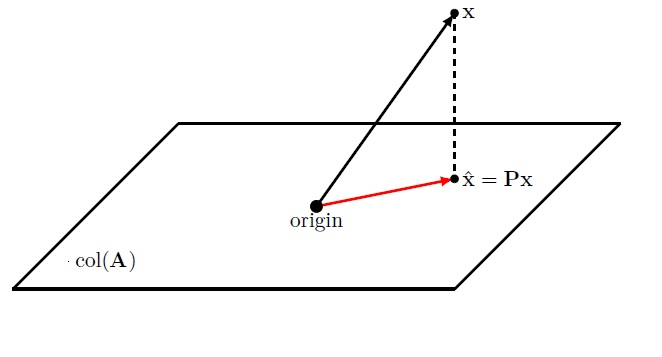
\includegraphics[scale=0.5]{fig2.jpg}
	\caption{Geometric illustration of the orthogonal projection operator $P$. A vector $x \in R^m$ is restricted to the column space of $A$, where $Px \in col(A)$.}
	\label{fig2}
\end{figure}


The concept of random projections can be used to sample the range (column space) of the input matrix $A$ in order to efficiently construct such a orthogonal projector. Random projections are data agnostic, and constructed by first drawing a set of $k$ random vectors ${[\omega_i]}_{i =1} ^{k}$ , for instance, from the standard normal distribution. Probability theory guarantees that random vectors are linearly independent with high probability. Then, a set of random projections ${[y_i]}_{i =1} ^{k}$ is computed by mapping $A$ to low-dimensional space:
\begin{equation}\label{eq1}
y_i = \mathbf{A}\omega _i,\ \ \ for\ i = 1...k
\end{equation}

In other words, this process forms a set of independent randomly weighted linear combinations of the columns of A, and reduces the number of columns from $n$ to $k$. While the input matrix is compressed, the Euclidean distances between the original data points are approximately preserved. Random projections are also well known as the Johnson-Lindenstrauss (JL) transform (Johnson and Lindenstrauss 1984).

Equation 3 can be efficiently executed in parallel. Therefore, let us define the random test matrix $\Omega \in R^{n \times k}$, which is again drawn from the standard normal distribution, and the columns of which are given by the vectors $\omega_i$. The samples matrix $Q \in R^{m \times k}$, also denoted as sketch, is then obtained by post-multiplying the input matrix by the random test matrix $ Y := A\Omega $
Once Y is obtained, it only remains to orthonormalize the columns in order to form a natural basis $Q \in R^{m \times k}$ This can be efficiently achieved using the QR-decomposition $Y =: QR$. 

\textit{Stage B: Compute the smaller matrix}

Now, given the near-optimal basis $Q$, we aim to find a smaller matrix $B \in R^{k \times n}$. Therefore, we project the high-dimensional input matrix $A$ to low-dimensional space 
\begin{equation}
B:= Q^T A
\end{equation}
Geometrically, this is a projection (i.e., a linear transformation) which takes points in a high-dimensional space into corresponding points in a low-dimensional space, illustrated in Figure 3.

\begin{figure}
	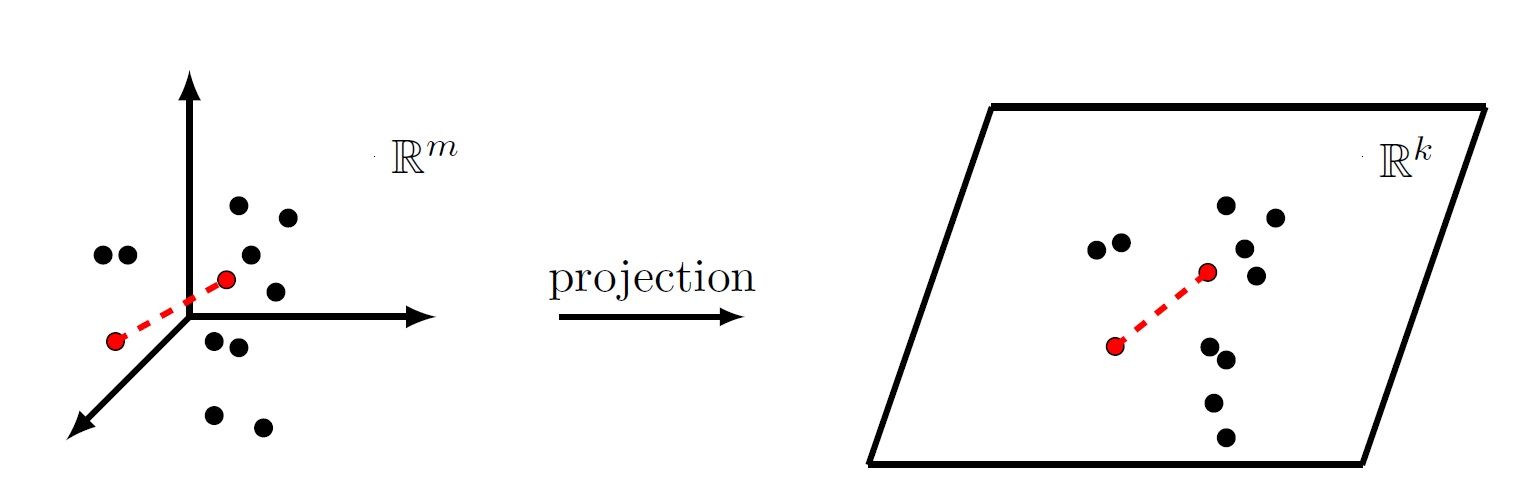
\includegraphics[scale=0.25]{fig3.jpg}
	\caption{Points in a high-dimensional space are projected into low-dimensional space, while
		the geometric structure is preserved in an Euclidean sense.}
	\label{fig3}
\end{figure}


This process preserves the geometric structure of the data in an Euclidean sense, i.e., the length of the projected vectors as well as the angles between the projected vectors are preserved. So finally we have:
\begin{equation}
A \approx Q B
\end{equation}

This decomposition is referred to as the $QB$ decomposition. Subsequently, the smaller matrix $B$ can be used to compute a matrix decomposition using a traditional algorithm.


\subsection{Improved randomized algorithm}
The basis matrix $Q$ often fails to provide a good approximation for the column space of the input matrix. This is because most real-world data matrices do not feature a precise rank $r$, and instead exhibit a gradually decaying singular value spectrum. The performance can be considerably improved using the concept of oversampling and the power iteration scheme.\\

\textit{Oversampling}\\ 
Most data matrices do not feature an exact rank. Oversampling can be used to overcome this issue by using more random projections to form the sketch, instead of just $k$. The intuition behind the oversampling scheme is the following. The sketch Y is a random variable, as it depends on the drawing of a random test matrix 
. Increasing the number of additional random projections allows one to decrease the variation in the singular value spectrum of the random test matrix, which subsequently improves the quality of the sketch.\\

\textit{Power iteration scheme}\\
The second method for improving the quality of the basis $Q$ involves the concept of power sampling iterations . Instead of obtaining the sketch $Y$ directly, the data matrix $A$ is first preprocessed as
\begin{equation}
A^{(q)} := (AA^T)^q A
\end{equation}
where $q$ is an integer specifying the number of power iterations. This process enforces a more rapid decay of the singular values. Thus, we enable the algorithm to sample the relevant information related to the dominant singular values, while unwanted information is suppressed. Finally the algorithm to calculate our randomized SVD is shown in Figure 4.

\begin{figure}
	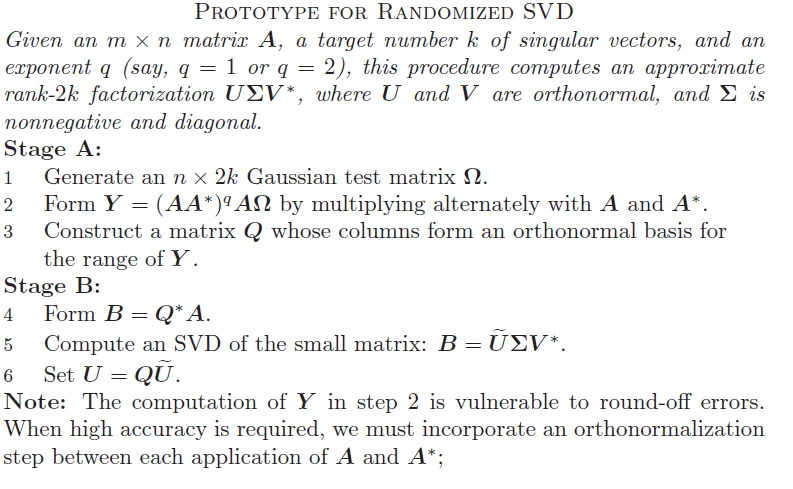
\includegraphics[scale=0.4]{fig4.jpg}
	\caption{The algorithm to calculate our randomized SVD.}
	\label{fig3}
\end{figure}

\subsection{Error Analysis and Number of Computation}
In this section we give bounds on the error of the proposed randomized SVD and find number of flops required to compute it.
\subsubsection{Error Analysis}
we refer to the theorem 2.1 by Halko et al. (2011) and restate it here for future use. \\
\textit{Theorem}\\
Suppose that $A$ is areal $m \times n$  matrix. select an exponent $q$ and a target number $k$ of singular vectors, where $2 \leq k \leq 0.5\min{(m, n)}$. Execute the randomized SVD algorithm to obtain a rank-$2k$ factorization of $U\Sigma V^*$ Then:
\begin{equation}
\mathbb{E} ||A-U\Sigma V^*|| \leq [1+4\sqrt{\frac{2\min{(m,n)}}{k-1}}]^{\frac{1}{2q}} \sigma_{k+1}
\end{equation}
where $\mathbb{E}$ denotes the expectation with respect to the random test matrix and $\sigma_{k+1}$ is the $(k+1)$th singular value of $A$. 

\subsubsection{Flops Count}
Number of flops required for traditional SVD is $\min(mn^2,nm^2)$, while in the randomized SVD we have $mn\log{k}+ k^2(m+n)$. when $k$ in much smaller than $m$ and $n$ it really beats traditional SVD.

 
\section{Examples}
The examples are provided in \textbf{Jupyter notebook}


\begin{thebibliography}{}


   \bibitem{cox} N. Halko, P. G. Martinsson, and J. A. Tropp,
\textit{Finding structure with randomness: Probabilistic algorithms for constructing approximate matrix decompositions} (SIAM Review 2011 53:2, 217-288) 

   \end{thebibliography}

\end{document}

